\section{Bonus : Envoi d'un courrier (3 points)}

Le tableau ci-dessous présente des tarifs d'envoi de courrier de la Poste (en 2009) :

\begin{center}
	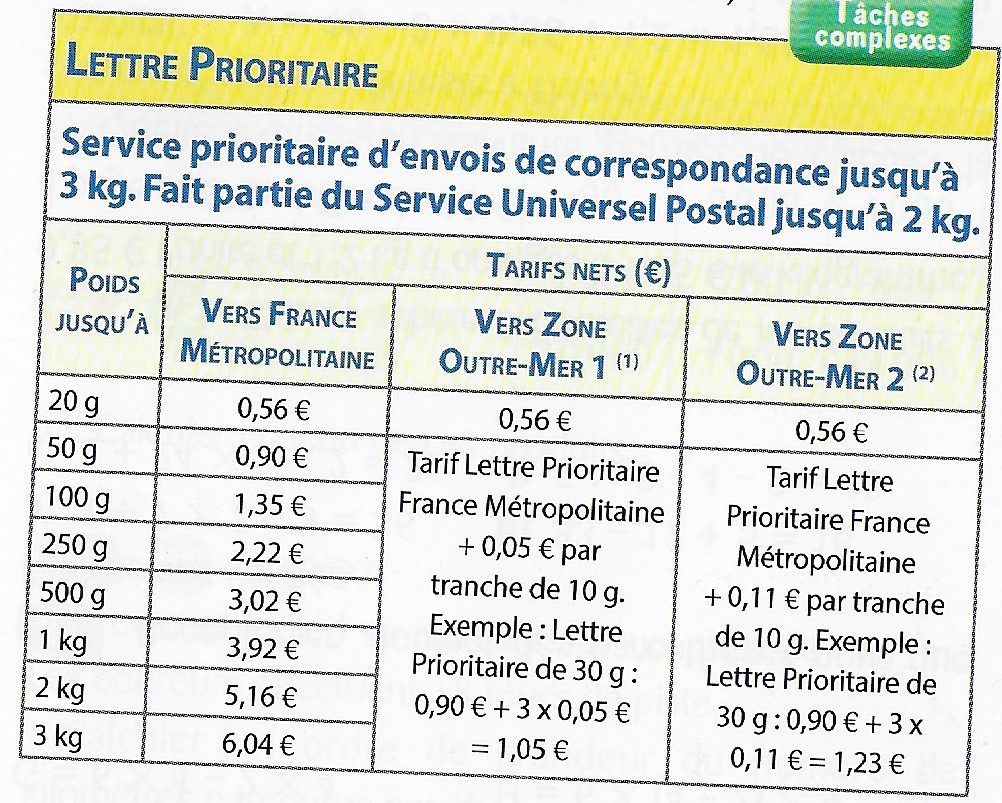
\includegraphics[scale=1.1]{img/poste}
\end{center}

\begin{questions}
	\question[1] Virginie envoie une lettre de 180 g vers la \textbf{Zone Outre-Mer 1}. Vérifier qu'elle va payer \num{3.12} €
	
	\question[1] Cathy envoie une lettre de 2 kg vers la \textbf{Zone Outre-Mer 2}. Combien va-t-elle payer ?
	
	\question[1] Théo poste une lettre pour la \textbf{Zone Outre-Mer 2}, il paye \num{6.32} €. Quelle est la masse maximale de sa lettre ?
	

\end{questions}